\documentclass[a4paper,11pt]{article}
\usepackage{mathpazo}
\usepackage{tikz}
\usetikzlibrary{shapes}
\oddsidemargin -0.54cm
\textwidth 17.00cm
\textheight 24cm
\topmargin -1.3cm
\parindent 0pt
\parskip 1ex
\pagestyle{empty}
\begin{document}
\medskip\hrule\medskip

0 0 2 0 2 2 4 0 2 -2 are inserted 

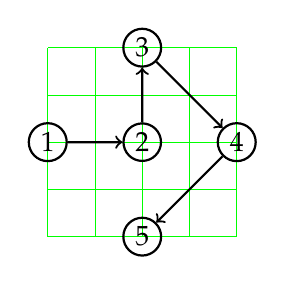
\begin{tikzpicture}[scale=0.600]
\draw [help lines, color=green] (0,-2) grid (4,2);

\draw [thick] (0,0) node[draw, rounded rectangle] (0) {1};
\draw [thick] (2,0) node[draw, rounded rectangle] (1) {2};
\draw [thick] (2,2) node[draw, rounded rectangle] (2) {3};
\draw [thick] (4,0) node[draw, rounded rectangle] (3) {4};
\draw [thick] (2,-2) node[draw, rounded rectangle] (4) {5};
\draw [->, thick] (0) to (1);
\draw [->, thick] (1) to (2);
\draw [->, thick] (2) to (3);
\draw [->, thick] (3) to (4);

\end{tikzpicture}

\medskip\hrule\medskip
\end{document}